\section{Preliminary: Truth Discovery}
\label{sec:preliminary}

\begin{figure}
	\centering
	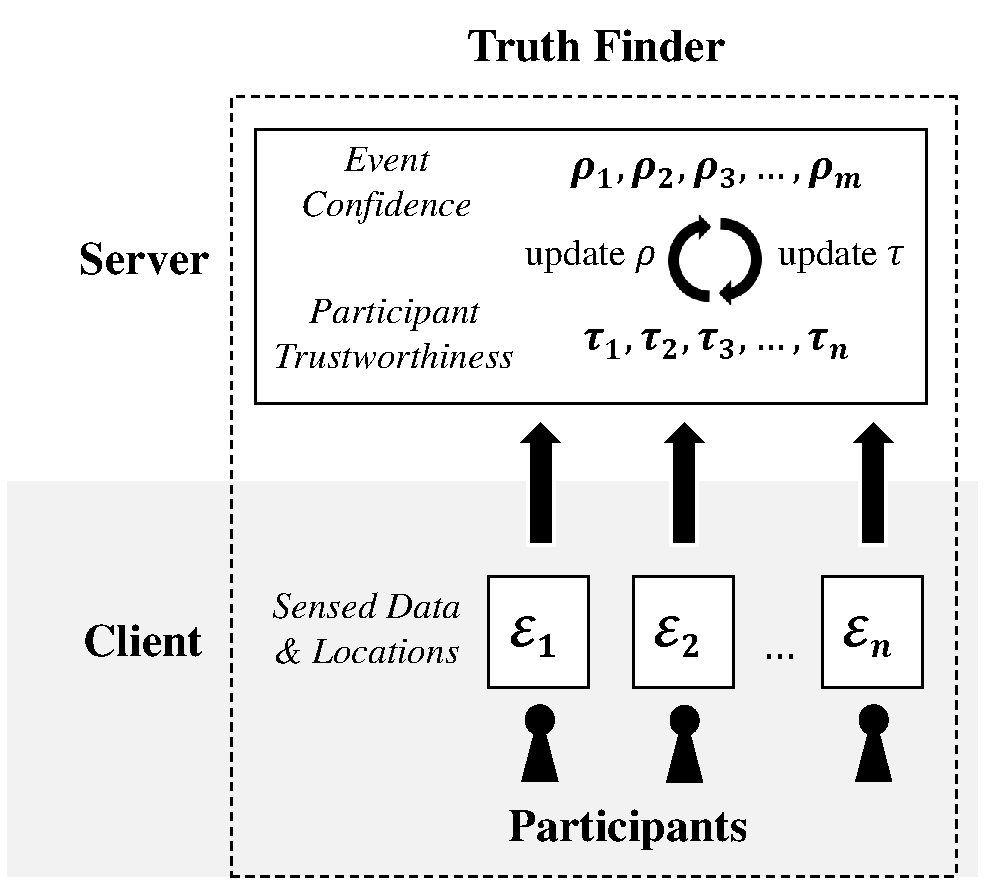
\includegraphics[width=.5\linewidth]{submissions/LeyeWang/fig/truthfinder.pdf}
	\caption{Overview of Iterative Truth Discovery}
	\label{fig:truthfinder}
	\vspace{-1em}
\end{figure}


Truth discovery algorithms usually follow an iterative method to calibrate user trustworthiness and data confidence alternatively until convergence \citep{yin2008truth}. Figure~\ref{fig:truthfinder} shows the framework of iterative truth discovery methods. In this paper, for clarity, we assume that sensed data is a binary spatial event. That is, for a specific location, the sensed data can be 1 or 0. Our method can be easily extended to multi-class and continuous-value events (see Appendix).

As shown in Figure~\ref{fig:truthfinder}, first, participants upload all of their sensed data and locations $\mathcal E_i$  to the central server. The central server would assign an initial trustworthiness score $\tau_i$ to each participant $u_i$ (e.g., 0.9 by assuming that 90\% of the sensed data are accurate). Then, for each sensed event $e_j$, the truth discovery algorithm will calculate its confidence $\rho_j$ (i.e., the probability of $e_j = 1$) by considering the users who have sensed $e_j$ as:
\begin{equation}
\rho_j = F_\rho(\mathcal U_{j,1}, \mathcal U_{j,0})
\label{eq:event_confidence}
\end{equation}
where $\mathcal U_{j,k}$ is the users who have sensed the event $e_j$ with the reported data $k$; $F_\rho$ is an event confidence calculation function which we will elaborate on later.

With $\rho_j$ for each event $e_j$, we can then update the trustworthiness score $\tau_i$ of each participant $u_i$ by:
\begin{equation}
\tau_i = F_\tau(\mathcal E_{i,1}, \mathcal E_{i,0})
\end{equation}
where $\mathcal E_{i,k}$ is the users' sensed event set with the reported data $k$; $F_\tau$ is a user trustworthiness calculation function which we will elaborate on later.

Once $\tau_i$ is updated for each user $u_i$, we can continue updating $\rho_j$ for each event $e_j$ according to Eq.~\ref{eq:event_confidence}, and so on, leading to an alternative updating process for both $\tau_i$ and $\rho_j$. This process can be terminated after a fixed number of iterations or until convergence. Next, we elaborate on the common choices of $F_\rho$ and $F_\tau$ in literature.

\textbf{Sum Function}

An intuitive selection of the updating functions of $F_\rho$ and $F_\tau$ is the weighted sum:
\begin{equation}
\rho_j = F_\rho(\mathcal U_{j,1}, \mathcal U_{j,0}) = \frac{\sum_{u_i \in \mathcal U_{j,1}} \tau_i}{\sum_{u_i \in \mathcal U_{j,1}} \tau_i + \sum_{u_k \in \mathcal U_{j,0}} \tau_k}
\label{eq:rho_function_sum}
\end{equation}
\begin{equation}
\tau_i = F_\tau(\mathcal E_{i,1}, \mathcal E_{i,0}) = \frac{\sum_{e_j \in \mathcal E_{i,1}} \rho_j + \sum_{e_k \in \mathcal E_{i,0}} 1-\rho_k}{|\mathcal E_{i,1}|+|\mathcal E_{i,0}|}
\label{eq:tau_function}
\end{equation}

\textbf{Logistic Function}

Another widely used updating function is the Logistic function \citep{yin2008truth}. Its basic idea is seeing every user independently, so that the probability of event happening, i.e., $e_j=1$, can be formulated as:
\begin{equation}
	\rho_j = 1 - \prod_{u_i \in \mathcal U_{j,1}} (1-\tau_i)
\end{equation}
As $1-\tau_i$ may often be small and multiplying many of them may lead to underflow, prior studies proposed to use the logarithm to define a log-trustworthiness score of $u_i$ as \citep{yin2008truth}:
\begin{equation}
	\tau_i^* = - \ln(1-\tau_i)
\end{equation}
Similarly, a log-confidence score of event $e_j$ is defined as:
\begin{equation}
	\rho_j^* = - \ln(1-\rho_i)
\end{equation}
Then, we can infer
\begin{equation}
	\rho_j^* = \sum_{u_i \in \mathcal U_{j,1}} \tau_i^*
\end{equation}
The above equation does not consider the users' trustworthiness who report $e_j=0$, and thus we refine it:
\begin{equation}
	\rho_j^* = \sum_{u_i \in \mathcal U_{j,1}} \tau_i^* - \sum_{u_k \in \mathcal U_{j,0}} \tau_k^*
\end{equation}
Finally, a logistic function is used to calculate the final confidence $\rho_j$ of event $e_j$ \citep{yin2008truth}:
\begin{equation}
	\rho_j = F_\rho(\mathcal U_{j,1}, \mathcal U_{j,0}) = (1+e^{-\rho_j^*})^{-1}
	\label{eq:rho_function_log}
\end{equation}
$\tau_i$ is updated same as Eq.~\ref{eq:tau_function}. 